\documentclass[11pt]{report}

\usepackage{graphicx}
\usepackage{listings}
\usepackage{color}

\setlength{\topmargin}{0in}
\setlength{\headheight}{0in}
\setlength{\headsep}{0in}
\setlength{\textheight}{9.0in}
\setlength{\textwidth}{6.5in}
\setlength{\evensidemargin}{0in}
\setlength{\oddsidemargin}{0in}


\begin{document}

\title{Revisions to MPAS data structures}
\author{}

\maketitle
\tableofcontents


%%%%%%%%%%%%%%%%%%%%%%%%%%%%%%%%%%%%%%%%
%
% Introduction
%
%%%%%%%%%%%%%%%%%%%%%%%%%%%%%%%%%%%%%%%%
\chapter{Introduction}

In order to support multiple blocks of cells per MPI task, there are a number of
development issues that need to be addressed:

\begin{enumerate}

\item Update/extend the fundamental derived types in mpas\_grid\_types.F.                                
   In order for other parts of the infrastructure to handle multiple                                
   blocks per task in a clean way, we'll need to be able to pass a head                             
   pointer to a field into a routine, and have that routine loop through                            
   all blocks for that field, with information about which cells/edges/vertices                     
   in that field need to be communicated.                                                           
                                                                                                    
\item Decide on a new MPAS I/O abstraction layer, which will provide a                                
   high-level interface to the PIO layer for the rest of MPAS. This layer                           
   should work with blocks of fields, and make it possible to define an                             
   arbitrary set of I/O streams at run-time.                                                        
                                                                                                    
\item Add a new module to parse a run-time I/O configuration file that                                
   will describe which fields are read or written to each of the I/O                                
   streams that a user requests via the file. This module will make calls                           
   to the new MPAS I/O layer to register the requested fields for I/O in                            
   the requested streams.                                          
   
\item Update the mpas\_dmpar module to support communication operations on                              
   multiple blocks per task. This will likely involve revising the                                  
   internal data structures used to define communication of cells                                   
   between tasks, and also require revisions to the public interface                                
   routines themselves.                                                                             
                                                                                                    
\item Modify the block\_decomp module to enable a task to get a list of                                 
   cells in more than one block that it is to be the owner of.                                      
   Implemented in the simplest way, there could simply be a namelist                                
   option to specify how many blocks each task should own, and the                                  
   block\_decomp module could look for a graph.info.part.n file, with                                
   n=num\_blocks\_per\_task*num\_tasks, and assign blocks k, 2k, 3k, ...,                               
   num\_blocks\_per\_task*k to task k.    

\end{enumerate}                                                             
                                                                                                    
This document concerns the first item, namely, the extensions to the derived data
types that will be necessary for supporting multiple blocks per task in other infrastructure
modules.       


%%%%%%%%%%%%%%%%%%%%%%%%%%%%%%%%%%%%%%%%
%
% Requirements
%
%%%%%%%%%%%%%%%%%%%%%%%%%%%%%%%%%%%%%%%%
\chapter{Requirements}

The changes to the derived data types used throughout the MPAS infrastructure and cores
should enable I/O, communication, and other infrastructure routines to elegantly handle multiple blocks per MPI task.

\begin{itemize}

\item Routines (e.g., operators) must be able to traverse the list of blocks for any field that is owned by a task without having
to explicitly dereference that field by name; this ensures that infrastructure routines can remain generic.

\item A block for a field must be able to access the parallel information (halo communication lists, as well as
MPI communicator) associated with it so that such information is never explicitly passed with the field
to infrastructure subroutines. This requirement will simplify the argument lists for infrastructure routines, and 
eliminate the possibility that a user might pass mismatched or invalid communication information for a field
to an infrastructure routine.

\item A field must be aware of its dimensions and other metadata so that such information is never explicitly 
passed with the field to infrastructure subroutines, thereby eliminating the possibility that a user might pass incorrect dimensions
for a field, for example.

\item Since halo updates may require exchanges between blocks owned by the same process, the data
structures used by the halo update routines (and other routines in mpas\_dmpar.F) must distinguish between
halo cells in other blocks owned by the MPI task from those in blocks owned by a different MPI task.

\item Though not strictly related to supporting multiple blocks per MPI task, halo update data structures should
enable halo exchange routines to easily exchange any subset of the ghost cell layers. This may enable efficiency
gains to be made in future.

\end{itemize}



%%%%%%%%%%%%%%%%%%%%%%%%%%%%%%%%%%%%%%%%
%
% Design
%
%%%%%%%%%%%%%%%%%%%%%%%%%%%%%%%%%%%%%%%%
\chapter{Design}

We propose to extend the existing data structures in MPAS with additional pointers
between fields of the same type, and also with pointers within fields to the appropriate communication
lists for that field. The set of communications lists will be extended to include separate lists for inter-process
(distributed memory) and intra-process (shared-memory) exchanges, and each list will identify cells/edges/vertices
to be exchanged for a single layer of ghost cells/edges/vertices, necessitating one list per halo layer. Also, additional metadata 
will be carried around within each field type. The proposed changes 
are highlighted in the field type definition below; other type definitions are given for reference, and the figure below 
illustrates graphically the hierarchy of DDTs.

\begin{figure}[htb]
\begin{center}
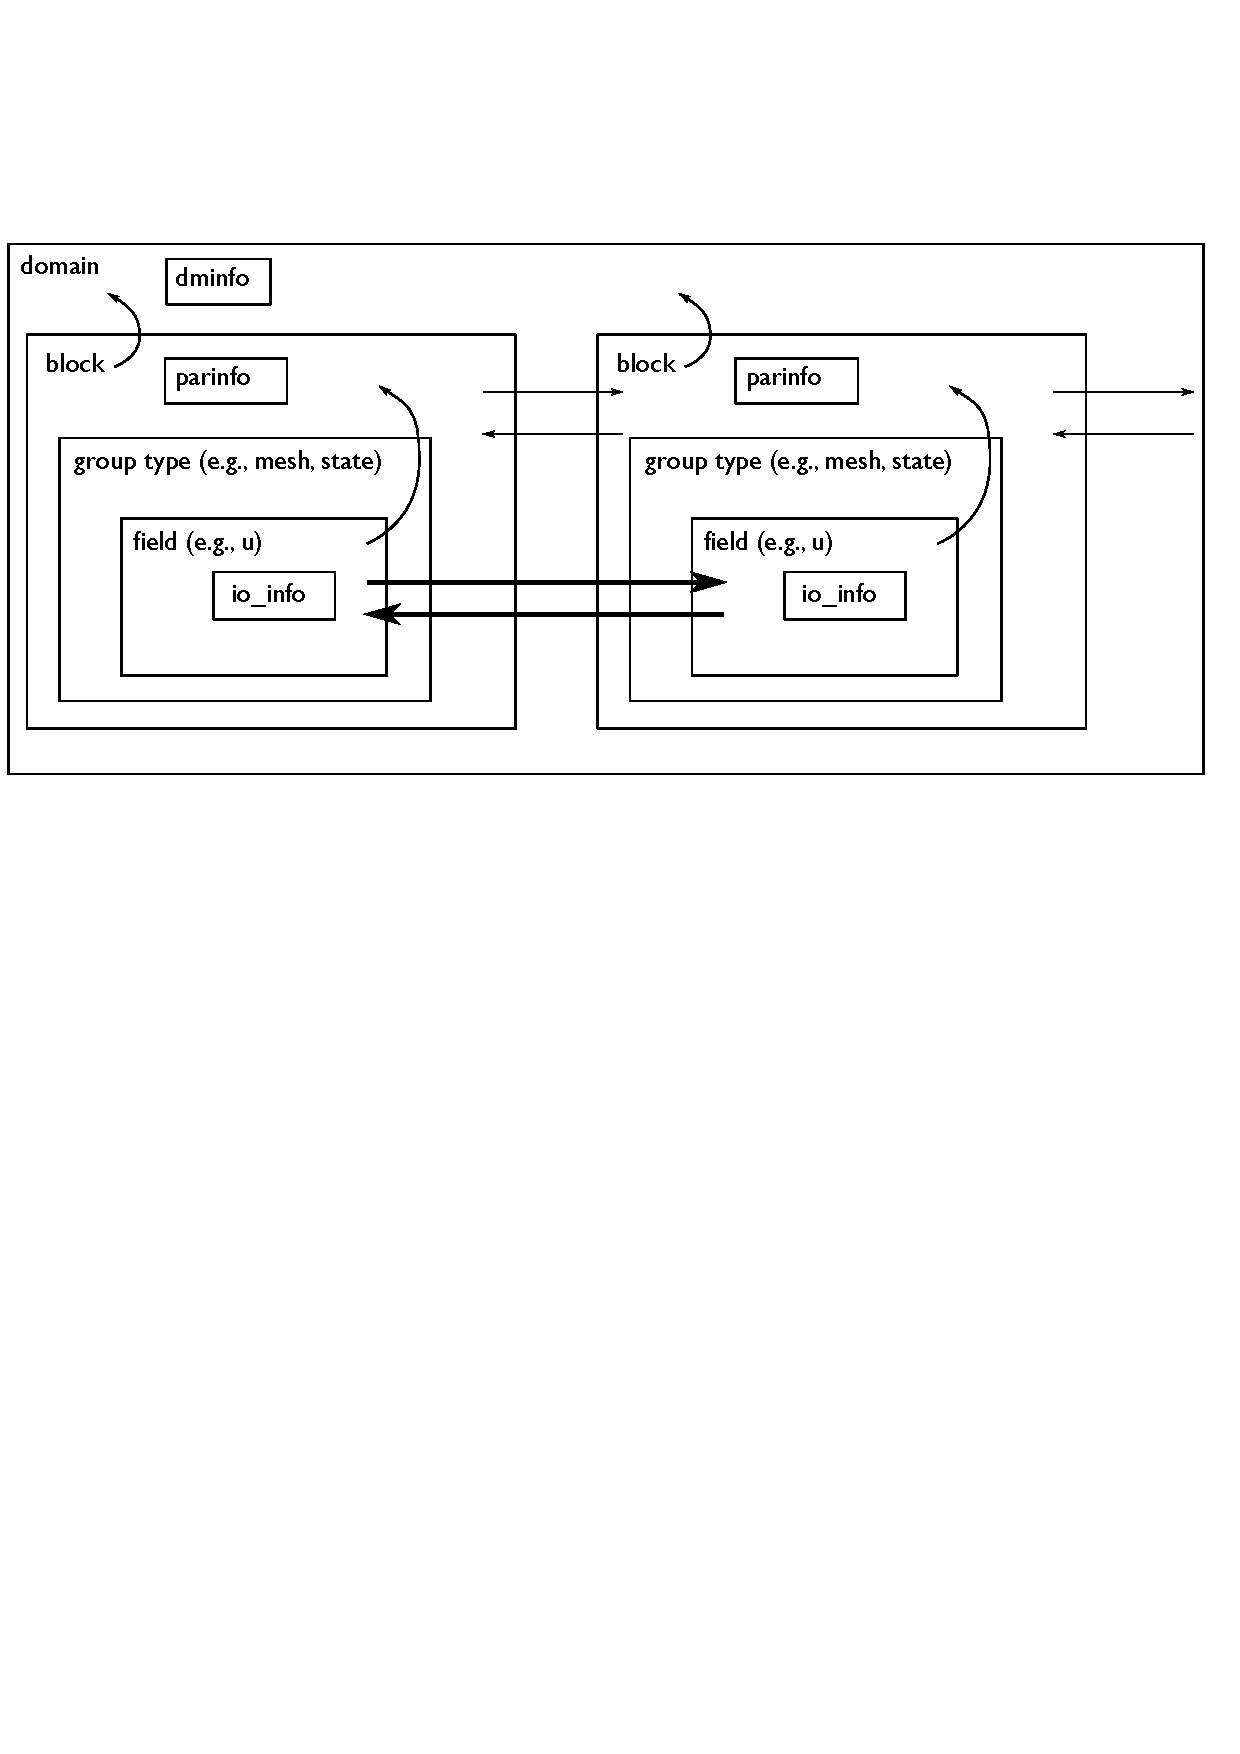
\includegraphics[width=6.5in]{ddt_reorg.pdf}
\caption{An illustration of the current DDT structure: existing back-pointers and previous/next pointers are drawn in light arrows; new pointers to be added between field blocks are drawn heavy arrows.}
\end{center}
\end{figure}

Besides the simple additions to the derived types described here, we will also need to extend
the infrastructure routines that deal with allocating, deallocating, and reading in fields to be aware that there may be multiple
blocks for a field; however, this work will be addressed by work on items 2, 4, and 5 identified in the Introduction to this document.
\pagebreak

\begin{lstlisting}[language=fortran,escapechar=@,frame=single]
! Derived type for storing list of blocks from a domain 
! to be handled by a process
type domain_type
   type (block_type), pointer :: blocklist

   ! Also store parallelization info here
   type (dm_info), pointer :: dminfo
end type domain_type
\end{lstlisting}

\begin{lstlisting}[language=fortran,escapechar=@,frame=single]
type dm_info
   integer :: nprocs, my_proc_id, comm, info
end type dm_info
\end{lstlisting}
\vspace{12pt}

In the block\_type, we will need to add a global block ID number, which uniquely identifies
the block within the global block space. This will be used for both intra-process halo copies, as well
as inter-process halo messages (in conjunction with the process ID that owns the block). 
\linebreak

\begin{lstlisting}[language=fortran,escapechar=@,frame=single]
! Derived type for storing part of a domain; used as a basic 
! unit of work for a process
type block_type

#include "block_group_members.inc"

   type (domain_type), pointer :: domain

   type (parallel_info), pointer :: parinfo
   
    @\colorbox{yellow}{integer :: blockID}@

   type (block_type), pointer :: prev, next
end type block_type
\end{lstlisting}

\begin{lstlisting}[language=fortran,escapechar=@,frame=single]
type exchange_list
   integer :: procID
   @\colorbox{yellow}{integer :: blockID}@
   integer :: nlist
   integer, dimension(:), pointer :: list
   type (exchange_list), pointer :: next
   real (kind=RKIND), dimension(:), pointer :: rbuffer
   integer, dimension(:), pointer           :: ibuffer
   integer :: reqID
end type exchange_list
\end{lstlisting}   
\vspace{12pt}

In the parallel\_info type, the existing (inter-process) exchange lists will become arrays, 
with the first index of the array providing an exchange list for the first halo layer, the second
index for the second halo layer, etc. For example, cellsToSend(2) and cellsToRecv(2) give 
information about which cells should be sent and received for a block to update the second
(outer) halo layer. For cells, the interpretation of ``first halo layer'', ``second halo layer'', etc.
are obvious, but we need to carefully define the interpretation of ``layers'' for edges and 
vertices. We propose that the first halo layer for edges refers to the set of ghost edges bordering owned cells, 
the second halo layer refers to the set of ghost edges bordering first halo cells, etc., and similarly
for vertices.
\linebreak

\begin{lstlisting}[language=fortran,escapechar=@,frame=single]
! Type for storing (possibly architecture specific) information 
! concerning parallelism
type parallel_info
   type (exchange_list), @\colorbox{yellow}{dimension(:),}@ pointer :: cellsToSend    
   type (exchange_list), @\colorbox{yellow}{dimension(:),}@ pointer :: cellsToRecv 
   @\colorbox{yellow}{type (exchange\_list), dimension(:), pointer :: cellsToCopy}@ 
    
   type (exchange_list), @\colorbox{yellow}{dimension(:),}@ pointer :: edgesToSend    
   type (exchange_list), @\colorbox{yellow}{dimension(:),}@ pointer :: edgesToRecv 
   @\colorbox{yellow}{type (exchange\_list), dimension(:), pointer :: edgesToCopy}@    
   
   type (exchange_list), @\colorbox{yellow}{dimension(:),}@ pointer :: verticesToSend      
   type (exchange_list), @\colorbox{yellow}{dimension(:),}@ pointer :: verticesToRecv
   @\colorbox{yellow}{type (exchange\_list), dimension(:), pointer :: verticesToCopy}@
    
end type parallel_info
\end{lstlisting}
\vspace{12pt}

Each field will carry around its dimensions, as well as whether it has a time dimension in input
and output files, pointers to the previous and next block for the field, and pointers to the exchange
lists for the field; if the field is a non-decomposed field, the exchange pointers will be nullified.
\linebreak

\begin{lstlisting}[language=fortran,escapechar=@,frame=single]
! Derived type for storing fields
type field3DReal
   type (block_type), pointer :: block
   real (kind=RKIND), dimension(:,:,:), pointer :: array
   type (io_info), pointer :: ioinfo
   @\colorbox{yellow}{integer, dimension(3) :: dims}@
   @\colorbox{yellow}{logical :: timeDimension}@
   @\colorbox{yellow}{type (field3DReal), pointer :: prev, next}@
   @\colorbox{yellow}{type (exchange\_list), dimension(:), pointer :: sendList}@
   @\colorbox{yellow}{type (exchange\_list), dimension(:), pointer :: recvList}@
   @\colorbox{yellow}{type (exchange\_list), dimension(:), pointer :: copyList}@
end type field3DReal
\end{lstlisting}
\vspace{12pt}

The io\_info type will be extended to contain units and description information for the field.
\linebreak

\begin{lstlisting}[language=fortran,escapechar=@,frame=single]
! Derived type describing info for doing I/O specific to a field
type io_info
   character (len=1024) :: fieldName
   @\colorbox{yellow}{character (len=1024) :: units}@
   @\colorbox{yellow}{character (len=1024) :: description}@
   integer, dimension(4) :: start
   integer, dimension(4) :: count
   logical :: input
   logical :: sfc
   logical :: restart
   logical :: output
end type io_info
\end{lstlisting}


%%%%%%%%%%%%%%%%%%%%%%%%%%%%%%%%%%%%%%%%
%
% Implementation
%
%%%%%%%%%%%%%%%%%%%%%%%%%%%%%%%%%%%%%%%%
\chapter{Implementation}

Should we outline a plan for implementing these changes?

\end{document}
